% Options for packages loaded elsewhere
\PassOptionsToPackage{unicode}{hyperref}
\PassOptionsToPackage{hyphens}{url}
\PassOptionsToPackage{dvipsnames,svgnames,x11names}{xcolor}
%
\documentclass[
  letterpaper,
  DIV=11,
  numbers=noendperiod]{scrreprt}

\usepackage{amsmath,amssymb}
\usepackage{iftex}
\ifPDFTeX
  \usepackage[T1]{fontenc}
  \usepackage[utf8]{inputenc}
  \usepackage{textcomp} % provide euro and other symbols
\else % if luatex or xetex
  \usepackage{unicode-math}
  \defaultfontfeatures{Scale=MatchLowercase}
  \defaultfontfeatures[\rmfamily]{Ligatures=TeX,Scale=1}
\fi
\usepackage{lmodern}
\ifPDFTeX\else  
    % xetex/luatex font selection
\fi
% Use upquote if available, for straight quotes in verbatim environments
\IfFileExists{upquote.sty}{\usepackage{upquote}}{}
\IfFileExists{microtype.sty}{% use microtype if available
  \usepackage[]{microtype}
  \UseMicrotypeSet[protrusion]{basicmath} % disable protrusion for tt fonts
}{}
\makeatletter
\@ifundefined{KOMAClassName}{% if non-KOMA class
  \IfFileExists{parskip.sty}{%
    \usepackage{parskip}
  }{% else
    \setlength{\parindent}{0pt}
    \setlength{\parskip}{6pt plus 2pt minus 1pt}}
}{% if KOMA class
  \KOMAoptions{parskip=half}}
\makeatother
\usepackage{xcolor}
\setlength{\emergencystretch}{3em} % prevent overfull lines
\setcounter{secnumdepth}{5}
% Make \paragraph and \subparagraph free-standing
\ifx\paragraph\undefined\else
  \let\oldparagraph\paragraph
  \renewcommand{\paragraph}[1]{\oldparagraph{#1}\mbox{}}
\fi
\ifx\subparagraph\undefined\else
  \let\oldsubparagraph\subparagraph
  \renewcommand{\subparagraph}[1]{\oldsubparagraph{#1}\mbox{}}
\fi

\usepackage{color}
\usepackage{fancyvrb}
\newcommand{\VerbBar}{|}
\newcommand{\VERB}{\Verb[commandchars=\\\{\}]}
\DefineVerbatimEnvironment{Highlighting}{Verbatim}{commandchars=\\\{\}}
% Add ',fontsize=\small' for more characters per line
\usepackage{framed}
\definecolor{shadecolor}{RGB}{241,243,245}
\newenvironment{Shaded}{\begin{snugshade}}{\end{snugshade}}
\newcommand{\AlertTok}[1]{\textcolor[rgb]{0.68,0.00,0.00}{#1}}
\newcommand{\AnnotationTok}[1]{\textcolor[rgb]{0.37,0.37,0.37}{#1}}
\newcommand{\AttributeTok}[1]{\textcolor[rgb]{0.40,0.45,0.13}{#1}}
\newcommand{\BaseNTok}[1]{\textcolor[rgb]{0.68,0.00,0.00}{#1}}
\newcommand{\BuiltInTok}[1]{\textcolor[rgb]{0.00,0.23,0.31}{#1}}
\newcommand{\CharTok}[1]{\textcolor[rgb]{0.13,0.47,0.30}{#1}}
\newcommand{\CommentTok}[1]{\textcolor[rgb]{0.37,0.37,0.37}{#1}}
\newcommand{\CommentVarTok}[1]{\textcolor[rgb]{0.37,0.37,0.37}{\textit{#1}}}
\newcommand{\ConstantTok}[1]{\textcolor[rgb]{0.56,0.35,0.01}{#1}}
\newcommand{\ControlFlowTok}[1]{\textcolor[rgb]{0.00,0.23,0.31}{#1}}
\newcommand{\DataTypeTok}[1]{\textcolor[rgb]{0.68,0.00,0.00}{#1}}
\newcommand{\DecValTok}[1]{\textcolor[rgb]{0.68,0.00,0.00}{#1}}
\newcommand{\DocumentationTok}[1]{\textcolor[rgb]{0.37,0.37,0.37}{\textit{#1}}}
\newcommand{\ErrorTok}[1]{\textcolor[rgb]{0.68,0.00,0.00}{#1}}
\newcommand{\ExtensionTok}[1]{\textcolor[rgb]{0.00,0.23,0.31}{#1}}
\newcommand{\FloatTok}[1]{\textcolor[rgb]{0.68,0.00,0.00}{#1}}
\newcommand{\FunctionTok}[1]{\textcolor[rgb]{0.28,0.35,0.67}{#1}}
\newcommand{\ImportTok}[1]{\textcolor[rgb]{0.00,0.46,0.62}{#1}}
\newcommand{\InformationTok}[1]{\textcolor[rgb]{0.37,0.37,0.37}{#1}}
\newcommand{\KeywordTok}[1]{\textcolor[rgb]{0.00,0.23,0.31}{#1}}
\newcommand{\NormalTok}[1]{\textcolor[rgb]{0.00,0.23,0.31}{#1}}
\newcommand{\OperatorTok}[1]{\textcolor[rgb]{0.37,0.37,0.37}{#1}}
\newcommand{\OtherTok}[1]{\textcolor[rgb]{0.00,0.23,0.31}{#1}}
\newcommand{\PreprocessorTok}[1]{\textcolor[rgb]{0.68,0.00,0.00}{#1}}
\newcommand{\RegionMarkerTok}[1]{\textcolor[rgb]{0.00,0.23,0.31}{#1}}
\newcommand{\SpecialCharTok}[1]{\textcolor[rgb]{0.37,0.37,0.37}{#1}}
\newcommand{\SpecialStringTok}[1]{\textcolor[rgb]{0.13,0.47,0.30}{#1}}
\newcommand{\StringTok}[1]{\textcolor[rgb]{0.13,0.47,0.30}{#1}}
\newcommand{\VariableTok}[1]{\textcolor[rgb]{0.07,0.07,0.07}{#1}}
\newcommand{\VerbatimStringTok}[1]{\textcolor[rgb]{0.13,0.47,0.30}{#1}}
\newcommand{\WarningTok}[1]{\textcolor[rgb]{0.37,0.37,0.37}{\textit{#1}}}

\providecommand{\tightlist}{%
  \setlength{\itemsep}{0pt}\setlength{\parskip}{0pt}}\usepackage{longtable,booktabs,array}
\usepackage{calc} % for calculating minipage widths
% Correct order of tables after \paragraph or \subparagraph
\usepackage{etoolbox}
\makeatletter
\patchcmd\longtable{\par}{\if@noskipsec\mbox{}\fi\par}{}{}
\makeatother
% Allow footnotes in longtable head/foot
\IfFileExists{footnotehyper.sty}{\usepackage{footnotehyper}}{\usepackage{footnote}}
\makesavenoteenv{longtable}
\usepackage{graphicx}
\makeatletter
\def\maxwidth{\ifdim\Gin@nat@width>\linewidth\linewidth\else\Gin@nat@width\fi}
\def\maxheight{\ifdim\Gin@nat@height>\textheight\textheight\else\Gin@nat@height\fi}
\makeatother
% Scale images if necessary, so that they will not overflow the page
% margins by default, and it is still possible to overwrite the defaults
% using explicit options in \includegraphics[width, height, ...]{}
\setkeys{Gin}{width=\maxwidth,height=\maxheight,keepaspectratio}
% Set default figure placement to htbp
\makeatletter
\def\fps@figure{htbp}
\makeatother
\newlength{\cslhangindent}
\setlength{\cslhangindent}{1.5em}
\newlength{\csllabelwidth}
\setlength{\csllabelwidth}{3em}
\newlength{\cslentryspacingunit} % times entry-spacing
\setlength{\cslentryspacingunit}{\parskip}
\newenvironment{CSLReferences}[2] % #1 hanging-ident, #2 entry spacing
 {% don't indent paragraphs
  \setlength{\parindent}{0pt}
  % turn on hanging indent if param 1 is 1
  \ifodd #1
  \let\oldpar\par
  \def\par{\hangindent=\cslhangindent\oldpar}
  \fi
  % set entry spacing
  \setlength{\parskip}{#2\cslentryspacingunit}
 }%
 {}
\usepackage{calc}
\newcommand{\CSLBlock}[1]{#1\hfill\break}
\newcommand{\CSLLeftMargin}[1]{\parbox[t]{\csllabelwidth}{#1}}
\newcommand{\CSLRightInline}[1]{\parbox[t]{\linewidth - \csllabelwidth}{#1}\break}
\newcommand{\CSLIndent}[1]{\hspace{\cslhangindent}#1}

\KOMAoption{captions}{tableheading}
\makeatletter
\makeatother
\makeatletter
\@ifpackageloaded{bookmark}{}{\usepackage{bookmark}}
\makeatother
\makeatletter
\@ifpackageloaded{caption}{}{\usepackage{caption}}
\AtBeginDocument{%
\ifdefined\contentsname
  \renewcommand*\contentsname{Table of contents}
\else
  \newcommand\contentsname{Table of contents}
\fi
\ifdefined\listfigurename
  \renewcommand*\listfigurename{List of Figures}
\else
  \newcommand\listfigurename{List of Figures}
\fi
\ifdefined\listtablename
  \renewcommand*\listtablename{List of Tables}
\else
  \newcommand\listtablename{List of Tables}
\fi
\ifdefined\figurename
  \renewcommand*\figurename{Figure}
\else
  \newcommand\figurename{Figure}
\fi
\ifdefined\tablename
  \renewcommand*\tablename{Table}
\else
  \newcommand\tablename{Table}
\fi
}
\@ifpackageloaded{float}{}{\usepackage{float}}
\floatstyle{ruled}
\@ifundefined{c@chapter}{\newfloat{codelisting}{h}{lop}}{\newfloat{codelisting}{h}{lop}[chapter]}
\floatname{codelisting}{Listing}
\newcommand*\listoflistings{\listof{codelisting}{List of Listings}}
\makeatother
\makeatletter
\@ifpackageloaded{caption}{}{\usepackage{caption}}
\@ifpackageloaded{subcaption}{}{\usepackage{subcaption}}
\makeatother
\makeatletter
\@ifpackageloaded{tcolorbox}{}{\usepackage[skins,breakable]{tcolorbox}}
\makeatother
\makeatletter
\@ifundefined{shadecolor}{\definecolor{shadecolor}{rgb}{.97, .97, .97}}
\makeatother
\makeatletter
\makeatother
\makeatletter
\makeatother
\ifLuaTeX
  \usepackage{selnolig}  % disable illegal ligatures
\fi
\IfFileExists{bookmark.sty}{\usepackage{bookmark}}{\usepackage{hyperref}}
\IfFileExists{xurl.sty}{\usepackage{xurl}}{} % add URL line breaks if available
\urlstyle{same} % disable monospaced font for URLs
\hypersetup{
  pdftitle={SOCI 3440},
  pdfauthor={John McLevey},
  colorlinks=true,
  linkcolor={blue},
  filecolor={Maroon},
  citecolor={Blue},
  urlcolor={Blue},
  pdfcreator={LaTeX via pandoc}}

\title{SOCI 3440}
\author{John McLevey}
\date{2024-09-17}

\begin{document}
\maketitle
\ifdefined\Shaded\renewenvironment{Shaded}{\begin{tcolorbox}[boxrule=0pt, interior hidden, frame hidden, borderline west={3pt}{0pt}{shadecolor}, enhanced, sharp corners, breakable]}{\end{tcolorbox}}\fi

\renewcommand*\contentsname{Table of contents}
{
\hypersetup{linkcolor=}
\setcounter{tocdepth}{2}
\tableofcontents
}
\bookmarksetup{startatroot}

\hypertarget{course-information}{%
\chapter*{Course Information}\label{course-information}}
\addcontentsline{toc}{chapter}{Course Information}

\markboth{Course Information}{Course Information}

\hypertarget{description}{%
\section*{Description}\label{description}}
\addcontentsline{toc}{section}{Description}

\markright{Description}

\hypertarget{schedule}{%
\section*{Schedule}\label{schedule}}
\addcontentsline{toc}{section}{Schedule}

\markright{Schedule}

\bookmarksetup{startatroot}

\hypertarget{telling-stories-with-data}{%
\chapter{Telling Stories with Data}\label{telling-stories-with-data}}

\bookmarksetup{startatroot}

\hypertarget{drinking-from-the-firehose}{%
\chapter{Drinking from the Firehose}\label{drinking-from-the-firehose}}

\begin{quote}
This notebook translates the R code in
\href{https://tellingstorieswithdata.com/02-drinking_from_a_fire_hose.html}{Chapter
2: Drinking from the Firehose} to Python.
\end{quote}

\hypertarget{examples-in-python}{%
\section{Examples in Python}\label{examples-in-python}}

\hypertarget{setup}{%
\section{Setup}\label{setup}}

\begin{Shaded}
\begin{Highlighting}[]
\ImportTok{import}\NormalTok{ pandas }\ImportTok{as}\NormalTok{ pd}
\ImportTok{from}\NormalTok{ io }\ImportTok{import}\NormalTok{ StringIO}
\ImportTok{import}\NormalTok{ numpy }\ImportTok{as}\NormalTok{ np}
\ImportTok{import}\NormalTok{ seaborn }\ImportTok{as}\NormalTok{ sns}
\ImportTok{import}\NormalTok{ matplotlib.pyplot }\ImportTok{as}\NormalTok{ plt}
\ImportTok{from}\NormalTok{ janitor }\ImportTok{import}\NormalTok{ clean\_names, remove\_empty}
\ImportTok{from}\NormalTok{ datetime }\ImportTok{import}\NormalTok{ datetime, timedelta}
\ImportTok{from}\NormalTok{ TorontoOpenData }\ImportTok{import}\NormalTok{ TorontoOpenData}
\ImportTok{import}\NormalTok{ requests}

\ImportTok{from}\NormalTok{ qrm3440 }\ImportTok{import}\NormalTok{ set\_style}
\NormalTok{set\_style()}
\end{Highlighting}
\end{Shaded}

\begin{verbatim}
/root/.cache/pypoetry/virtualenvs/qrm3440-djWU9zOu-py3.12/lib/python3.12/site-packages/ckanapi/version.py:1: DeprecationWarning: pkg_resources is deprecated as an API. See https://setuptools.pypa.io/en/latest/pkg_resources.html
  import pkg_resources
\end{verbatim}

\hypertarget{australian-elections}{%
\section{Australian Elections}\label{australian-elections}}

\hypertarget{simulate}{%
\subsection{Simulate}\label{simulate}}

\begin{Shaded}
\begin{Highlighting}[]
\NormalTok{np.random.seed(}\DecValTok{853}\NormalTok{)}

\NormalTok{simulated\_election\_data }\OperatorTok{=}\NormalTok{ \{}
    \StringTok{"Division"}\NormalTok{: }\BuiltInTok{range}\NormalTok{(}\DecValTok{1}\NormalTok{, }\DecValTok{152}\NormalTok{),}
    \StringTok{"Party"}\NormalTok{: np.random.choice(}
\NormalTok{        [}\StringTok{"Liberal"}\NormalTok{, }\StringTok{"Labour"}\NormalTok{, }\StringTok{"National"}\NormalTok{, }\StringTok{"Green"}\NormalTok{, }\StringTok{"Other"}\NormalTok{],}
\NormalTok{        size }\OperatorTok{=} \DecValTok{151}\NormalTok{,}
\NormalTok{        replace }\OperatorTok{=} \VariableTok{True}
\NormalTok{    )}
\NormalTok{\}}

\NormalTok{simulated\_election\_data }\OperatorTok{=}\NormalTok{ pd.DataFrame(simulated\_election\_data)}
\NormalTok{simulated\_election\_data.sample(}\DecValTok{10}\NormalTok{)}
\end{Highlighting}
\end{Shaded}

\begin{longtable}[]{@{}lll@{}}
\toprule\noalign{}
& Division & Party \\
\midrule\noalign{}
\endhead
\bottomrule\noalign{}
\endlastfoot
118 & 119 & Other \\
121 & 122 & National \\
104 & 105 & Liberal \\
132 & 133 & National \\
136 & 137 & Other \\
23 & 24 & Other \\
107 & 108 & National \\
56 & 57 & Liberal \\
101 & 102 & Green \\
93 & 94 & Liberal \\
\end{longtable}

\hypertarget{acquire}{%
\subsection{Acquire}\label{acquire}}

\begin{Shaded}
\begin{Highlighting}[]
\NormalTok{data\_url }\OperatorTok{=} \StringTok{"https://results.aec.gov.au/27966/website/Downloads/HouseMembersElectedDownload{-}27966.csv"}

\NormalTok{raw\_elections\_data }\OperatorTok{=}\NormalTok{ pd.read\_csv(data\_url, skiprows}\OperatorTok{=}\DecValTok{1}\NormalTok{)}
\NormalTok{raw\_elections\_data.to\_csv(}\StringTok{"data/australian\_voting.csv"}\NormalTok{, index}\OperatorTok{=}\VariableTok{False}\NormalTok{)}

\NormalTok{raw\_elections\_data.info()}
\end{Highlighting}
\end{Shaded}

\begin{verbatim}
<class 'pandas.core.frame.DataFrame'>
RangeIndex: 151 entries, 0 to 150
Data columns (total 8 columns):
 #   Column       Non-Null Count  Dtype 
---  ------       --------------  ----- 
 0   DivisionID   151 non-null    int64 
 1   DivisionNm   151 non-null    object
 2   StateAb      151 non-null    object
 3   CandidateID  151 non-null    int64 
 4   GivenNm      151 non-null    object
 5   Surname      151 non-null    object
 6   PartyNm      151 non-null    object
 7   PartyAb      151 non-null    object
dtypes: int64(2), object(6)
memory usage: 9.6+ KB
\end{verbatim}

\begin{Shaded}
\begin{Highlighting}[]
\NormalTok{raw\_elections\_data.sample(}\DecValTok{10}\NormalTok{)}
\end{Highlighting}
\end{Shaded}

\begin{longtable}[]{@{}lllllllll@{}}
\toprule\noalign{}
& DivisionID & DivisionNm & StateAb & CandidateID & GivenNm & Surname &
PartyNm & PartyAb \\
\midrule\noalign{}
\endhead
\bottomrule\noalign{}
\endlastfoot
41 & 252 & Dickson & QLD & 37493 & Peter & DUTTON & Liberal National
Party of Queensland & LNP \\
31 & 112 & Cook & NSW & 37025 & Scott & MORRISON & Liberal & LP \\
45 & 117 & Eden-Monaro & NSW & 36803 & Kristy & McBAIN & Australian
Labor Party & ALP \\
71 & 165 & Herbert & QLD & 37471 & Phillip & THOMPSON & Liberal National
Party of Queensland & LNP \\
131 & 250 & Riverina & NSW & 36324 & Michael & McCORMACK & The Nationals
& NP \\
50 & 161 & Fisher & QLD & 37504 & Andrew & WALLACE & Liberal National
Party of Queensland & LNP \\
39 & 158 & Dawson & QLD & 37485 & Andrew & WILLCOX & Liberal National
Party of Queensland & LNP \\
106 & 315 & McMahon & NSW & 36815 & Chris & BOWEN & Australian Labor
Party & ALP \\
133 & 177 & Ryan & QLD & 37370 & Elizabeth & WATSON-BROWN & The Greens &
GRN \\
81 & 219 & Isaacs & VIC & 36434 & Mark & DREYFUS & Australian Labor
Party & ALP \\
\end{longtable}

We can do a bit of cleaning using \texttt{janitor}.

\begin{Shaded}
\begin{Highlighting}[]
\NormalTok{cleaned\_elections\_data }\OperatorTok{=}\NormalTok{ clean\_names(raw\_elections\_data)}
\BuiltInTok{print}\NormalTok{(cleaned\_elections\_data.head(}\DecValTok{10}\NormalTok{))}
\end{Highlighting}
\end{Shaded}

\begin{verbatim}
   divisionid divisionnm stateab  candidateid           givennm    surname  \
0         179   Adelaide      SA        36973             Steve  GEORGANAS   
1         197      Aston     VIC        36704              Alan      TUDGE   
2         198   Ballarat     VIC        36409         Catherine       KING   
3         103      Banks     NSW        37018             David    COLEMAN   
4         180     Barker      SA        37083              Tony      PASIN   
5         104     Barton     NSW        36820             Linda     BURNEY   
6         192       Bass     TAS        37134  Bridget Kathleen     ARCHER   
7         318       Bean     ACT        36231             David      SMITH   
8         200    Bendigo     VIC        36424              Lisa   CHESTERS   
9         105  Bennelong     NSW        36827            Jerome     LAXALE   

                  partynm partyab  
0  Australian Labor Party     ALP  
1                 Liberal      LP  
2  Australian Labor Party     ALP  
3                 Liberal      LP  
4                 Liberal      LP  
5  Australian Labor Party     ALP  
6                 Liberal      LP  
7  Australian Labor Party     ALP  
8  Australian Labor Party     ALP  
9  Australian Labor Party     ALP  
\end{verbatim}

\begin{Shaded}
\begin{Highlighting}[]
\NormalTok{cleaned\_elections\_data }\OperatorTok{=}\NormalTok{ cleaned\_elections\_data[[}\StringTok{"divisionnm"}\NormalTok{, }\StringTok{"partynm"}\NormalTok{]]}

\NormalTok{cleaned\_elections\_data.sample(}\DecValTok{10}\NormalTok{)}
\end{Highlighting}
\end{Shaded}

\begin{longtable}[]{@{}lll@{}}
\toprule\noalign{}
& divisionnm & partynm \\
\midrule\noalign{}
\endhead
\bottomrule\noalign{}
\endlastfoot
0 & Adelaide & Australian Labor Party \\
2 & Ballarat & Australian Labor Party \\
50 & Fisher & Liberal National Party of Queensland \\
142 & Wannon & Liberal \\
49 & Fenner & Australian Labor Party \\
92 & Lingiari & Australian Labor Party \\
65 & Greenway & Australian Labor Party \\
9 & Bennelong & Australian Labor Party \\
69 & Hasluck & Australian Labor Party \\
119 & O\textquotesingle Connor & Liberal \\
\end{longtable}

\begin{Shaded}
\begin{Highlighting}[]
\BuiltInTok{print}\NormalTok{(cleaned\_elections\_data.columns)}

\NormalTok{cleaned\_elections\_data }\OperatorTok{=}\NormalTok{ cleaned\_elections\_data.rename(columns}\OperatorTok{=}\NormalTok{\{}
    \StringTok{"divisionnm"}\NormalTok{: }\StringTok{"division"}\NormalTok{,}
    \StringTok{"partynm"}\NormalTok{: }\StringTok{"elected\_party"}
\NormalTok{\})}

\NormalTok{cleaned\_elections\_data.sample(}\DecValTok{10}\NormalTok{)}
\end{Highlighting}
\end{Shaded}

\begin{verbatim}
Index(['divisionnm', 'partynm'], dtype='object')
\end{verbatim}

\begin{longtable}[]{@{}lll@{}}
\toprule\noalign{}
& division & elected\_party \\
\midrule\noalign{}
\endhead
\bottomrule\noalign{}
\endlastfoot
32 & Cooper & Australian Labor Party \\
16 & Braddon & Liberal \\
129 & Reid & Australian Labor Party \\
128 & Rankin & Australian Labor Party \\
33 & Corangamite & Australian Labor Party \\
11 & Blair & Australian Labor Party \\
57 & Fraser & Australian Labor Party \\
45 & Eden-Monaro & Australian Labor Party \\
109 & Menzies & Liberal \\
21 & Burt & Australian Labor Party \\
\end{longtable}

\begin{Shaded}
\begin{Highlighting}[]
\NormalTok{cleaned\_elections\_data[}\StringTok{"elected\_party"}\NormalTok{].unique()}
\end{Highlighting}
\end{Shaded}

\begin{verbatim}
array(['Australian Labor Party', 'Liberal',
       'Liberal National Party of Queensland', 'The Greens',
       'The Nationals', 'Independent', "Katter's Australian Party (KAP)",
       'Centre Alliance'], dtype=object)
\end{verbatim}

\begin{Shaded}
\begin{Highlighting}[]
\NormalTok{party\_map }\OperatorTok{=}\NormalTok{ \{}
    \StringTok{"Australian Labor Party"}\NormalTok{: }\StringTok{"Labor"}\NormalTok{,}
    \StringTok{"Liberal National Party of Queensland"}\NormalTok{: }\StringTok{"Liberal"}\NormalTok{,}
    \StringTok{"Liberal"}\NormalTok{: }\StringTok{"Liberal"}\NormalTok{,}
    \StringTok{"The Nationals"}\NormalTok{: }\StringTok{"Nationals"}\NormalTok{,}
    \StringTok{"The Greens"}\NormalTok{: }\StringTok{"Greens"}\NormalTok{,}
    \StringTok{"Independent"}\NormalTok{: }\StringTok{"Other"}\NormalTok{,}
    \StringTok{"Katter\textquotesingle{}s Australian Party (KAP)"}\NormalTok{: }\StringTok{"Other"}\NormalTok{,}
    \StringTok{"Centre Alliance"}\NormalTok{: }\StringTok{"Other"}
\NormalTok{\}}

\NormalTok{cleaned\_elections\_data[}\StringTok{"elected\_party"}\NormalTok{] }\OperatorTok{=}\NormalTok{ cleaned\_elections\_data[}\StringTok{"elected\_party"}\NormalTok{].}\BuiltInTok{map}\NormalTok{(party\_map)}

\NormalTok{cleaned\_elections\_data.head()}
\end{Highlighting}
\end{Shaded}

\begin{longtable}[]{@{}lll@{}}
\toprule\noalign{}
& division & elected\_party \\
\midrule\noalign{}
\endhead
\bottomrule\noalign{}
\endlastfoot
0 & Adelaide & Labor \\
1 & Aston & Liberal \\
2 & Ballarat & Labor \\
3 & Banks & Liberal \\
4 & Barker & Liberal \\
\end{longtable}

\begin{Shaded}
\begin{Highlighting}[]
\NormalTok{cleaned\_elections\_data.to\_csv(}\StringTok{"data/cleaned\_elections\_data.csv"}\NormalTok{, index}\OperatorTok{=}\VariableTok{False}\NormalTok{)}
\end{Highlighting}
\end{Shaded}

\hypertarget{explore}{%
\subsection{Explore}\label{explore}}

\begin{Shaded}
\begin{Highlighting}[]
\NormalTok{cleaned\_elections\_data }\OperatorTok{=}\NormalTok{ pd.read\_csv(}\StringTok{"data/cleaned\_elections\_data.csv"}\NormalTok{)}
\end{Highlighting}
\end{Shaded}

\begin{Shaded}
\begin{Highlighting}[]
\NormalTok{cleaned\_elections\_data[}\StringTok{"elected\_party"}\NormalTok{].value\_counts()}
\end{Highlighting}
\end{Shaded}

\begin{verbatim}
elected_party
Labor        77
Liberal      48
Other        12
Nationals    10
Greens        4
Name: count, dtype: int64
\end{verbatim}

Let's create our first plot!

\begin{Shaded}
\begin{Highlighting}[]
\NormalTok{plt.figure(figsize}\OperatorTok{=}\NormalTok{(}\DecValTok{10}\NormalTok{, }\DecValTok{6}\NormalTok{))}

\NormalTok{sns.countplot(}
\NormalTok{    x}\OperatorTok{=}\StringTok{"elected\_party"}\NormalTok{, }
\NormalTok{    data}\OperatorTok{=}\NormalTok{cleaned\_elections\_data}
\NormalTok{)}

\NormalTok{plt.title(}\StringTok{"No. of seats won by political party}\CharTok{\textbackslash{}n}\StringTok{in the 2022 Australian Federal Election}\CharTok{\textbackslash{}n}\StringTok{"}\NormalTok{, loc}\OperatorTok{=}\StringTok{\textquotesingle{}left\textquotesingle{}}\NormalTok{)}

\NormalTok{plt.xlabel(}\StringTok{""}\NormalTok{)}
\NormalTok{plt.ylabel(}\StringTok{"Number of seats}\CharTok{\textbackslash{}n}\StringTok{"}\NormalTok{)}

\NormalTok{plt.tight\_layout()}

\NormalTok{plt.savefig(}
    \StringTok{\textquotesingle{}figures/australian\_election\_2022.png\textquotesingle{}}\NormalTok{, dpi}\OperatorTok{=}\DecValTok{300}
\NormalTok{)}
\end{Highlighting}
\end{Shaded}

\begin{verbatim}
/usr/lib/python3.12/site-packages/IPython/core/pylabtools.py:77: DeprecationWarning: backend2gui is deprecated since IPython 8.24, backends are managed in matplotlib and can be externally registered.
  warnings.warn(
/usr/lib/python3.12/site-packages/IPython/core/pylabtools.py:77: DeprecationWarning: backend2gui is deprecated since IPython 8.24, backends are managed in matplotlib and can be externally registered.
  warnings.warn(
/tmp/ipykernel_4236/2891693074.py:13: UserWarning: The figure layout has changed to tight
  plt.tight_layout()
\end{verbatim}

\begin{verbatim}
/usr/lib/python3.12/site-packages/IPython/core/pylabtools.py:77: DeprecationWarning: backend2gui is deprecated since IPython 8.24, backends are managed in matplotlib and can be externally registered.
  warnings.warn(
\end{verbatim}

\begin{figure}[H]

{\centering 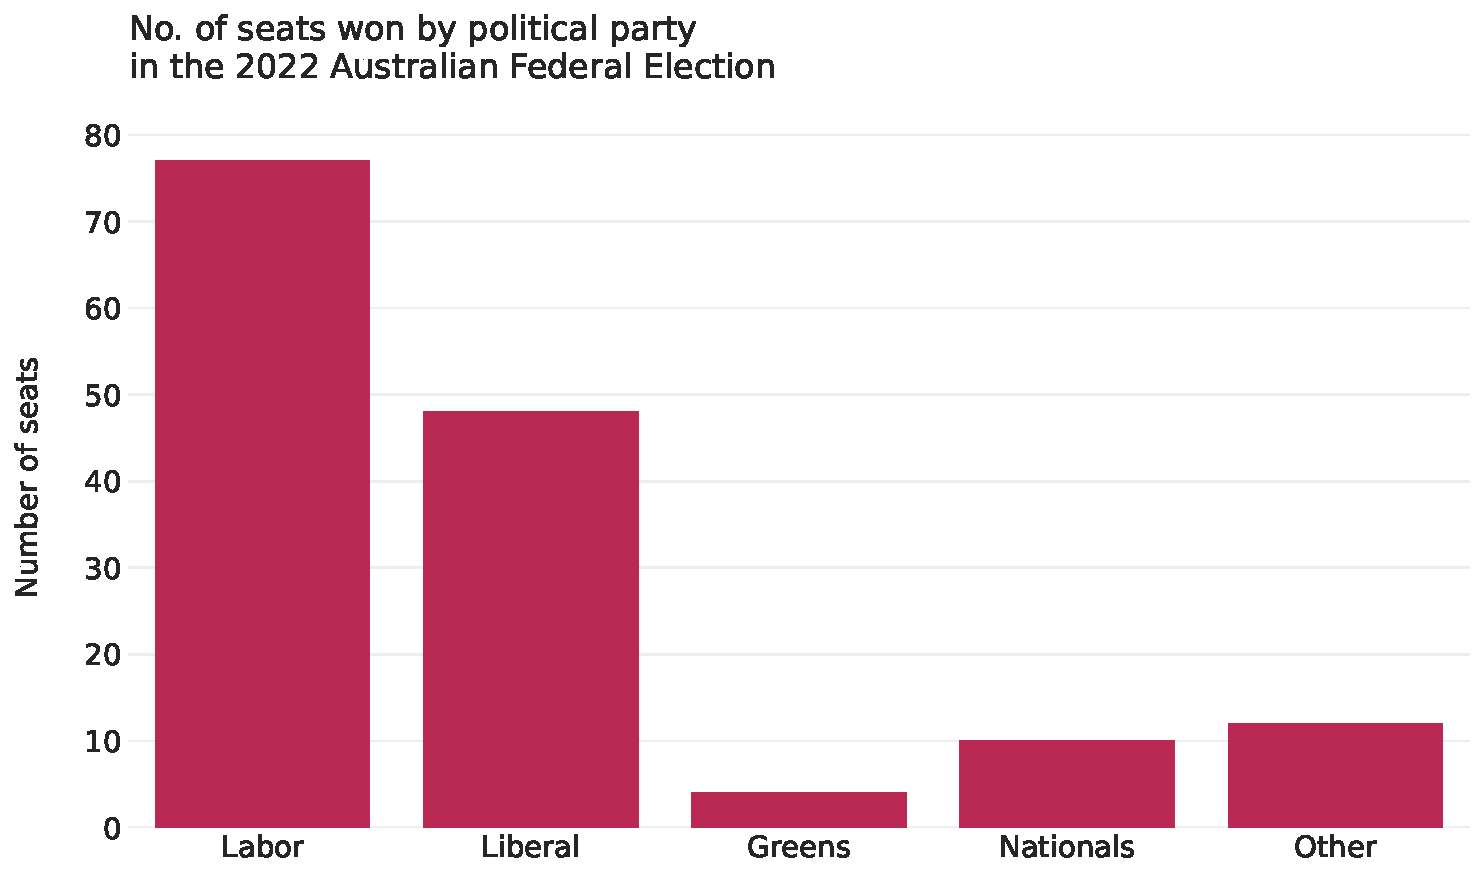
\includegraphics{firehose_files/figure-pdf/cell-14-output-3.pdf}

}

\end{figure}

\hypertarget{share}{%
\subsection{Share}\label{share}}

\begin{quote}
Australia is a parliamentary democracy with 151 seats in the House of
Representatives, which is the house from which government is formed.
There are two major parties---``Liberal'' and ``Labor''---two minor
parties---``Nationals'' and ``Greens''---and many smaller parties. The
2022 Federal Election occurred on 21 May, and around 15 million votes
were cast. We were interested in the number of seats that were won by
each party. We downloaded the results, on a seat-specific basis, from
the Australian Electoral Commission website. We cleaned and tidied the
dataset using Python and libraries including pandas, numpy, matplotlib,
and seaborn. We then created a graph of the number of seats that each
political party won. We found that the Labor Party won 77 seats,
followed by the Liberal Party with 48 seats. The minor parties won the
following number of seats: the Nationals won 10 seats and the Greens won
4 seats. Finally, there were 10 Independents elected as well as
candidates from smaller parties. The distribution of seats is skewed
toward the two major parties which could reflect relatively stable
preferences on the part of Australian voters, or possibly inertia due to
the benefits of already being a major party such a national network or
funding. A better understanding of the reasons for this distribution are
of interest in future work. While the dataset consists of everyone who
voted, it worth noting that in Australia some are systematically
excluded from voting, and it is much more difficult for some to vote
than others.
\end{quote}

\hypertarget{torontos-unhoused-population}{%
\section{Toronto's unhoused
population}\label{torontos-unhoused-population}}

\hypertarget{simulate-1}{%
\subsection{Simulate}\label{simulate-1}}

\begin{Shaded}
\begin{Highlighting}[]
\NormalTok{np.random.seed(}\DecValTok{853}\NormalTok{)}

\NormalTok{start\_date }\OperatorTok{=}\NormalTok{ datetime(}\DecValTok{2021}\NormalTok{, }\DecValTok{1}\NormalTok{, }\DecValTok{1}\NormalTok{)}
\NormalTok{dates }\OperatorTok{=}\NormalTok{ [start\_date }\OperatorTok{+}\NormalTok{ timedelta(days}\OperatorTok{=}\NormalTok{i) }\ControlFlowTok{for}\NormalTok{ i }\KeywordTok{in} \BuiltInTok{range}\NormalTok{(}\DecValTok{365}\NormalTok{)]}

\NormalTok{simulated\_occupancy\_data }\OperatorTok{=}\NormalTok{ pd.DataFrame(\{}
    \StringTok{\textquotesingle{}date\textquotesingle{}}\NormalTok{: dates }\OperatorTok{*} \DecValTok{3}\NormalTok{,}
    \StringTok{\textquotesingle{}shelter\textquotesingle{}}\NormalTok{: [}\StringTok{\textquotesingle{}Shelter 1\textquotesingle{}}\NormalTok{] }\OperatorTok{*} \DecValTok{365} \OperatorTok{+}\NormalTok{ [}\StringTok{\textquotesingle{}Shelter 2\textquotesingle{}}\NormalTok{] }\OperatorTok{*} \DecValTok{365} \OperatorTok{+}\NormalTok{ [}\StringTok{\textquotesingle{}Shelter 3\textquotesingle{}}\NormalTok{] }\OperatorTok{*} \DecValTok{365}\NormalTok{,}
    \StringTok{\textquotesingle{}number\_occupied\textquotesingle{}}\NormalTok{: np.random.poisson(lam}\OperatorTok{=}\DecValTok{30}\NormalTok{, size}\OperatorTok{=}\DecValTok{365}\OperatorTok{*}\DecValTok{3}\NormalTok{)}
\NormalTok{\})}

\NormalTok{simulated\_occupancy\_data.sample(}\DecValTok{10}\NormalTok{)}
\end{Highlighting}
\end{Shaded}

\begin{longtable}[]{@{}llll@{}}
\toprule\noalign{}
& date & shelter & number\_occupied \\
\midrule\noalign{}
\endhead
\bottomrule\noalign{}
\endlastfoot
1024 & 2021-10-22 & Shelter 3 & 31 \\
87 & 2021-03-29 & Shelter 1 & 24 \\
335 & 2021-12-02 & Shelter 1 & 34 \\
465 & 2021-04-11 & Shelter 2 & 25 \\
612 & 2021-09-05 & Shelter 2 & 29 \\
137 & 2021-05-18 & Shelter 1 & 40 \\
108 & 2021-04-19 & Shelter 1 & 21 \\
279 & 2021-10-07 & Shelter 1 & 34 \\
286 & 2021-10-14 & Shelter 1 & 21 \\
713 & 2021-12-15 & Shelter 2 & 36 \\
\end{longtable}

\hypertarget{acquire-1}{%
\subsection{Acquire}\label{acquire-1}}

The data is available
\href{https://open.toronto.ca/dataset/daily-shelter-overnight-service-occupancy-capacity/}{here}.

\begin{Shaded}
\begin{Highlighting}[]
\NormalTok{tod }\OperatorTok{=}\NormalTok{ TorontoOpenData()}

\NormalTok{search\_results }\OperatorTok{=}\NormalTok{ tod.search\_datasets(}\StringTok{\textquotesingle{}daily{-}shelter{-}overnight{-}service{-}occupancy{-}capacity{-}2021\textquotesingle{}}\NormalTok{)}
\NormalTok{search\_results}
\end{Highlighting}
\end{Shaded}

\begin{longtable}[]{@{}llllllllllllllllllllll@{}}
\toprule\noalign{}
& author & author\_email & creator\_user\_id & dataset\_category &
date\_published & excerpt & formats & id & information\_url &
is\_retired & ... & type & version & resources & tags & groups &
relationships\_as\_subject & relationships\_as\_object & civic\_issues &
owner\_section & owner\_unit \\
\midrule\noalign{}
\endhead
\bottomrule\noalign{}
\endlastfoot
0 & tsssdata@toronto.ca & tsssdata@toronto.ca &
329e1506-b545-4fc7-a4ea-e614f220eea7 & Table & 2021-06-28
13:44:56.408963 & Daily occupancy and capacity data for City of ... &
JSON,CSV,XML & 21c83b32-d5a8-4106-a54f-010dbe49f6f2 &
https://www.toronto.ca/city-government/data-re... & false & ... &
dataset & None &
{[}\{\textquotesingle cache\_last\_updated\textquotesingle: None,
\textquotesingle cache\_url\textquotesingle: Non... &
{[}\{\textquotesingle display\_name\textquotesingle:
\textquotesingle shelter\textquotesingle,
\textquotesingle id\textquotesingle: \textquotesingle9863812a-8... &
{[}{]} & {[}{]} & {[}{]} & NaN & NaN & NaN \\
1 & tsssdata@toronto.ca & tsssdata@toronto.ca &
329e1506-b545-4fc7-a4ea-e614f220eea7 & Table & 2019-07-23
17:00:10.298196 & Daily occupancy of the City of Toronto shelters &
CSV,XML,JSON & 8a6eceb2-821b-4961-a29d-758f3087732d &
https://www.toronto.ca/community-people/housin... & true & ... & dataset
& None & {[}\{\textquotesingle cache\_last\_updated\textquotesingle:
None, \textquotesingle cache\_url\textquotesingle: Non... &
{[}\{\textquotesingle display\_name\textquotesingle:
\textquotesingle homeless\textquotesingle,
\textquotesingle id\textquotesingle: \textquotesingle3af3eb57-... &
{[}{]} & {[}{]} & {[}{]} & NaN & NaN & NaN \\
2 & tsssdata@toronto.ca & tsssdata@toronto.ca &
329e1506-b545-4fc7-a4ea-e614f220eea7 & Document & 2019-07-23
17:34:37.680334 & The data set contains the location of the shel... &
SHP,XLS & 24b2b6ff-35b9-481d-9eb6-ba2e5e8b4dfb &
http://www.toronto.ca/housing/about-hostel.htm & false & ... & dataset &
None & {[}\{\textquotesingle cache\_last\_updated\textquotesingle: None,
\textquotesingle cache\_url\textquotesingle: Non... &
{[}\{\textquotesingle display\_name\textquotesingle:
\textquotesingle homeless shelter\textquotesingle,
\textquotesingle id\textquotesingle: \textquotesingle3... & {[}{]} &
{[}{]} & {[}{]} & affordable\_housing & NaN & NaN \\
3 & tsssdata@toronto.ca & tsssdata@toronto.ca &
329e1506-b545-4fc7-a4ea-e614f220eea7 & Document & 2022-09-30
18:43:00.949324 & This dataset includes a summary of responses f... &
XLSX,XLS & 5793a972-40fb-4e07-bc98-57c00590907a &
https://www.toronto.ca/community-people/commun... & false & ... &
dataset & None &
{[}\{\textquotesingle cache\_last\_updated\textquotesingle: None,
\textquotesingle cache\_url\textquotesingle: Non... & {[}{]} & {[}{]} &
{[}{]} & {[}{]} & NaN & NaN & NaN \\
4 & bikelocker@toronto.ca & bikelocker@toronto.ca &
329e1506-b545-4fc7-a4ea-e614f220eea7 & Map & 2019-07-23 16:34:00.669785
& A geospatial file that shows where all of the ... &
CSV,SHP,JSON,GEOJSON,GPKG & 2c32f356-e0ff-4245-84ba-cc3dd71a5694 &
http://www.toronto.ca/cycling & false & ... & dataset & None &
{[}\{\textquotesingle cache\_last\_updated\textquotesingle: None,
\textquotesingle cache\_url\textquotesingle: Non... &
{[}\{\textquotesingle display\_name\textquotesingle:
\textquotesingle bicycle parking\textquotesingle,
\textquotesingle id\textquotesingle: \textquotesingle8a... & {[}{]} &
{[}{]} & {[}{]} & NaN & NaN & NaN \\
5 & tsssdata@toronto.ca & tsssdata@toronto.ca &
329e1506-b545-4fc7-a4ea-e614f220eea7 & Table & 2021-11-15 00:00:00 & The
report includes monthly data about people ... & JSON,CSV,XML &
ac77f532-f18b-427c-905c-4ae87ce69c93 &
https://www.toronto.ca/city-government/data-re... & false & ... &
dataset & None &
{[}\{\textquotesingle cache\_last\_updated\textquotesingle: None,
\textquotesingle cache\_url\textquotesingle: Non... &
{[}\{\textquotesingle display\_name\textquotesingle:
\textquotesingle affordable housing\textquotesingle,
\textquotesingle id\textquotesingle: ... & {[}{]} & {[}{]} & {[}{]} &
NaN & SPI (Service Planning and Integrity) & NaN \\
6 & opendata@toronto.ca & opendata@toronto.ca &
329e1506-b545-4fc7-a4ea-e614f220eea7 & Document & 2019-07-23
17:59:05.514613 & This dataset is a tabular file that outlines f... &
XLSX,XLS & 1643a780-b01c-4a1d-b6b3-2c0538d111b3 &
http://www.toronto.ca/housing/about-hostel.htm & false & ... & dataset &
None & {[}\{\textquotesingle cache\_last\_updated\textquotesingle: None,
\textquotesingle cache\_url\textquotesingle: Non... &
{[}\{\textquotesingle display\_name\textquotesingle:
\textquotesingle housing\textquotesingle,
\textquotesingle id\textquotesingle: \textquotesingle72f69466-9... &
{[}{]} & {[}{]} & {[}{]} & Affordable housing,Poverty reduction & NaN &
NaN \\
7 & Sandro.Tersigni@toronto.ca & Sandro.Tersigni@toronto.ca &
329e1506-b545-4fc7-a4ea-e614f220eea7 & Map & 2019-07-23 18:03:41.634773
& Transit shelter location and asset type data f... &
GPKG,CSV,SHP,GEOJSON & 1db34737-ffad-489d-a590-9171d500d453 & NaN &
false & ... & dataset & None &
{[}\{\textquotesingle cache\_last\_updated\textquotesingle: None,
\textquotesingle cache\_url\textquotesingle: Non... &
{[}\{\textquotesingle display\_name\textquotesingle:
\textquotesingle bus shelter\textquotesingle,
\textquotesingle id\textquotesingle: \textquotesingle ded095... & {[}{]}
& {[}{]} & {[}{]} & Mobility & NaN & NaN \\
8 & opendata@toronto.ca & opendata@toronto.ca &
329e1506-b545-4fc7-a4ea-e614f220eea7 & Website & 2019-07-23
17:00:02.089385 & Number of client visits to Daily Bread Food Ba... &
XLS,WEB & 2d48a61d-da9b-4cfb-9dac-19f65492f756 &
http://www.toronto.ca/progressportal & true & ... & dataset & None &
{[}\{\textquotesingle cache\_last\_updated\textquotesingle: None,
\textquotesingle cache\_url\textquotesingle: Non... &
{[}\{\textquotesingle display\_name\textquotesingle:
\textquotesingle daily bread food bank\textquotesingle,
\textquotesingle id... & {[}{]} & {[}{]} & {[}{]} & NaN & NaN & NaN \\
9 & animalservices@toronto.ca & animalservices@toronto.ca &
329e1506-b545-4fc7-a4ea-e614f220eea7 & Document & 2020-10-02
16:35:28.527043 & The data includes requests for service regardi... &
XLS & 694b6a00-7850-4d2b-a2f4-0d6ab93f8883 &
http://www.toronto.ca/animalservices & false & ... & dataset & None &
{[}\{\textquotesingle cache\_last\_updated\textquotesingle: None,
\textquotesingle cache\_url\textquotesingle: Non... &
{[}\{\textquotesingle display\_name\textquotesingle:
\textquotesingle animals\textquotesingle,
\textquotesingle id\textquotesingle: \textquotesingle183cf169-0... &
{[}{]} & {[}{]} & {[}{]} & NaN & Animal Services & Enforcement \& Mobile
Response \\
\end{longtable}

We can download the data we want using the \texttt{id}.

\begin{Shaded}
\begin{Highlighting}[]
\NormalTok{did }\OperatorTok{=} \StringTok{\textquotesingle{}21c83b32{-}d5a8{-}4106{-}a54f{-}010dbe49f6f2\textquotesingle{}}
\NormalTok{downloaded\_data }\OperatorTok{=}\NormalTok{ tod.download\_dataset(did)}

\NormalTok{downloaded\_data}
\end{Highlighting}
\end{Shaded}

\begin{verbatim}
  0%|          | 0/16 [00:00<?, ?it/s]
\end{verbatim}

\begin{verbatim}
100%|██████████| 16/16 [00:00<00:00, 5850.82it/s]
\end{verbatim}

\begin{verbatim}
File cache/21c83b32-d5a8-4106-a54f-010dbe49f6f2/Daily shelter overnight occupancy.csv already exists. Skipping...
File cache/21c83b32-d5a8-4106-a54f-010dbe49f6f2/Daily shelter overnight occupancy.xml already exists. Skipping...
File cache/21c83b32-d5a8-4106-a54f-010dbe49f6f2/Daily shelter overnight occupancy.json already exists. Skipping...
File cache/21c83b32-d5a8-4106-a54f-010dbe49f6f2/daily-shelter-overnight-service-occupancy-capacity-2022.csv already exists. Skipping...
File cache/21c83b32-d5a8-4106-a54f-010dbe49f6f2/daily-shelter-overnight-service-occupancy-capacity-2022.xml already exists. Skipping...
File cache/21c83b32-d5a8-4106-a54f-010dbe49f6f2/daily-shelter-overnight-service-occupancy-capacity-2022.json already exists. Skipping...
File cache/21c83b32-d5a8-4106-a54f-010dbe49f6f2/daily-shelter-overnight-service-occupancy-capacity-2021.csv already exists. Skipping...
File cache/21c83b32-d5a8-4106-a54f-010dbe49f6f2/daily-shelter-overnight-service-occupancy-capacity-2021.xml already exists. Skipping...
File cache/21c83b32-d5a8-4106-a54f-010dbe49f6f2/daily-shelter-overnight-service-occupancy-capacity-2021.json already exists. Skipping...
File cache/21c83b32-d5a8-4106-a54f-010dbe49f6f2/daily-shelter-overnight-service-occupancy-capacity-2023.csv already exists. Skipping...
File cache/21c83b32-d5a8-4106-a54f-010dbe49f6f2/daily-shelter-overnight-service-occupancy-capacity-2023.xml already exists. Skipping...
File cache/21c83b32-d5a8-4106-a54f-010dbe49f6f2/daily-shelter-overnight-service-occupancy-capacity-2023.json already exists. Skipping...

Downloaded 0 resources: []
\end{verbatim}

\begin{verbatim}
\end{verbatim}

\begin{Shaded}
\begin{Highlighting}[]
\NormalTok{dfn }\OperatorTok{=} \StringTok{"daily{-}shelter{-}overnight{-}service{-}occupancy{-}capacity{-}2021.csv"}
\NormalTok{toronto\_shelters\_2021 }\OperatorTok{=}\NormalTok{ tod.load(did, dfn, smart\_return}\OperatorTok{=}\VariableTok{True}\NormalTok{)}
\NormalTok{toronto\_shelters\_2021}
\end{Highlighting}
\end{Shaded}

\begin{longtable}[]{@{}llllllllllllllllllllll@{}}
\toprule\noalign{}
& \_id & OCCUPANCY\_DATE & ORGANIZATION\_ID & ORGANIZATION\_NAME &
SHELTER\_ID & SHELTER\_GROUP & LOCATION\_ID & LOCATION\_NAME &
LOCATION\_ADDRESS & LOCATION\_POSTAL\_CODE & ... & OCCUPIED\_BEDS &
UNOCCUPIED\_BEDS & UNAVAILABLE\_BEDS & CAPACITY\_ACTUAL\_ROOM &
CAPACITY\_FUNDING\_ROOM & OCCUPIED\_ROOMS & UNOCCUPIED\_ROOMS &
UNAVAILABLE\_ROOMS & OCCUPANCY\_RATE\_BEDS & OCCUPANCY\_RATE\_ROOMS \\
\midrule\noalign{}
\endhead
\bottomrule\noalign{}
\endlastfoot
0 & 1 & 21-01-01 & 24 & COSTI Immigrant Services & 40 & COSTI Reception
Centre & 1103.0 & COSTI/City North York West Hotel Program & 1677 Wilson
Ave & M3L 1A5 & ... & NaN & NaN & NaN & 29.0 & 58.0 & 26.0 & 3.0 & 29.0
& NaN & 89.66 \\
1 & 2 & 21-01-01 & 24 & COSTI Immigrant Services & 40 & COSTI Reception
Centre & 1103.0 & COSTI/City North York West Hotel Program & 1677 Wilson
Ave & M3L 1A5 & ... & NaN & NaN & NaN & 3.0 & 0.0 & 3.0 & 0.0 & 0.0 &
NaN & 100.00 \\
2 & 3 & 21-01-01 & 24 & COSTI Immigrant Services & 40 & COSTI Reception
Centre & 1103.0 & COSTI/City North York West Hotel Program & 1677 Wilson
Ave & M3L 1A5 & ... & NaN & NaN & NaN & 28.0 & 0.0 & 23.0 & 5.0 & 0.0 &
NaN & 82.14 \\
3 & 4 & 21-01-01 & 24 & COSTI Immigrant Services & 40 & COSTI Reception
Centre & 1103.0 & COSTI/City North York West Hotel Program & 1677 Wilson
Ave & M3L 1A5 & ... & NaN & NaN & NaN & 17.0 & 0.0 & 17.0 & 0.0 & 0.0 &
NaN & 100.00 \\
4 & 5 & 21-01-01 & 24 & COSTI Immigrant Services & 40 & COSTI Reception
Centre & 1103.0 & COSTI/City North York West Hotel Program & 1677 Wilson
Ave & M3L 1A5 & ... & NaN & NaN & NaN & 14.0 & 0.0 & 13.0 & 1.0 & 0.0 &
NaN & 92.86 \\
... & ... & ... & ... & ... & ... & ... & ... & ... & ... & ... & ... &
... & ... & ... & ... & ... & ... & ... & ... & ... & ... \\
50939 & 50940 & 21-12-31 & 17 & YWCA Toronto & 78 & YWCA-348 Davenport &
1129.0 & YWCA Davenport Shelter & 348 Davenport Road & M5R 1K6 & ... &
6.0 & 14.0 & 0.0 & NaN & NaN & NaN & NaN & NaN & 30.00 & NaN \\
50940 & 50941 & 21-12-31 & 31 & Youth Without Shelter & 52 & Youth
Without Shelter & 1064.0 & Youth Without Shelter & 6 Warrendale Ct & M9V
1P9 & ... & 23.0 & 0.0 & 0.0 & NaN & NaN & NaN & NaN & NaN & 100.00 &
NaN \\
50941 & 50942 & 21-12-31 & 31 & Youth Without Shelter & 52 & Youth
Without Shelter & 1064.0 & Youth Without Shelter & 6 Warrendale Ct & M9V
1P9 & ... & 13.0 & 1.0 & 0.0 & NaN & NaN & NaN & NaN & NaN & 92.86 &
NaN \\
50942 & 50943 & 21-12-31 & 38 & YouthLink & 81 & YouthLink Shelter &
1147.0 & YouthLink & 747 Warden Ave & M1L 4A1 & ... & 10.0 & 0.0 & 0.0 &
NaN & NaN & NaN & NaN & NaN & 100.00 & NaN \\
50943 & 50944 & 21-12-31 & 38 & YouthLink & 81 & YouthLink Shelter &
1147.0 & YouthLink & 747 Warden Ave & M1L 4A1 & ... & 29.0 & 0.0 & 2.0 &
NaN & NaN & NaN & NaN & NaN & 100.00 & NaN \\
\end{longtable}

\begin{Shaded}
\begin{Highlighting}[]
\NormalTok{toronto\_shelters\_clean }\OperatorTok{=}\NormalTok{ clean\_names(toronto\_shelters\_2021)}
\NormalTok{toronto\_shelters\_clean.columns}
\end{Highlighting}
\end{Shaded}

\begin{verbatim}
Index(['_id', 'occupancy_date', 'organization_id', 'organization_name',
       'shelter_id', 'shelter_group', 'location_id', 'location_name',
       'location_address', 'location_postal_code', 'location_city',
       'location_province', 'program_id', 'program_name', 'sector',
       'program_model', 'overnight_service_type', 'program_area',
       'service_user_count', 'capacity_type', 'capacity_actual_bed',
       'capacity_funding_bed', 'occupied_beds', 'unoccupied_beds',
       'unavailable_beds', 'capacity_actual_room', 'capacity_funding_room',
       'occupied_rooms', 'unoccupied_rooms', 'unavailable_rooms',
       'occupancy_rate_beds', 'occupancy_rate_rooms'],
      dtype='object')
\end{verbatim}

\begin{Shaded}
\begin{Highlighting}[]
\NormalTok{toronto\_shelters\_clean }\OperatorTok{=}\NormalTok{ toronto\_shelters\_clean[}
\NormalTok{    [}\StringTok{\textquotesingle{}occupancy\_date\textquotesingle{}}\NormalTok{, }\StringTok{\textquotesingle{}occupied\_beds\textquotesingle{}}\NormalTok{]}
\NormalTok{]}
\end{Highlighting}
\end{Shaded}

\begin{Shaded}
\begin{Highlighting}[]
\NormalTok{toronto\_shelters\_clean.to\_csv(}\StringTok{\textquotesingle{}data/toronto\_shelters\_clean.csv\textquotesingle{}}\NormalTok{, index}\OperatorTok{=}\VariableTok{False}\NormalTok{)}
\end{Highlighting}
\end{Shaded}

\hypertarget{explore-1}{%
\subsection{Explore}\label{explore-1}}

\begin{Shaded}
\begin{Highlighting}[]
\NormalTok{toronto\_shelters\_clean }\OperatorTok{=}\NormalTok{ pd.read\_csv(}
    \StringTok{"data/toronto\_shelters\_clean.csv"}
\NormalTok{)}

\NormalTok{toronto\_shelters\_clean[}\StringTok{\textquotesingle{}occupancy\_date\textquotesingle{}}\NormalTok{] }\OperatorTok{=}\NormalTok{ pd.to\_datetime(}
\NormalTok{    toronto\_shelters\_clean[}\StringTok{\textquotesingle{}occupancy\_date\textquotesingle{}}\NormalTok{],}
    \BuiltInTok{format}\OperatorTok{=}\StringTok{\textquotesingle{}\%y{-}\%m{-}}\SpecialCharTok{\%d}\StringTok{\textquotesingle{}}
\NormalTok{)}

\NormalTok{toronto\_shelters\_clean}
\end{Highlighting}
\end{Shaded}

\begin{longtable}[]{@{}lll@{}}
\toprule\noalign{}
& occupancy\_date & occupied\_beds \\
\midrule\noalign{}
\endhead
\bottomrule\noalign{}
\endlastfoot
0 & 2021-01-01 & NaN \\
1 & 2021-01-01 & NaN \\
2 & 2021-01-01 & NaN \\
3 & 2021-01-01 & NaN \\
4 & 2021-01-01 & NaN \\
... & ... & ... \\
50939 & 2021-12-31 & 6.0 \\
50940 & 2021-12-31 & 23.0 \\
50941 & 2021-12-31 & 13.0 \\
50942 & 2021-12-31 & 10.0 \\
50943 & 2021-12-31 & 29.0 \\
\end{longtable}

Monthly occupancy. Make this code look a little friendlier.

\begin{Shaded}
\begin{Highlighting}[]
\NormalTok{monthly\_occupancy }\OperatorTok{=}\NormalTok{ (}
\NormalTok{    toronto\_shelters\_clean}
\NormalTok{    .assign(occupancy\_month}\OperatorTok{=}\NormalTok{toronto\_shelters\_clean[}\StringTok{\textquotesingle{}occupancy\_date\textquotesingle{}}\NormalTok{].dt.strftime(}\StringTok{\textquotesingle{}\%B\textquotesingle{}}\NormalTok{))}
\NormalTok{    .sort\_values(}\StringTok{\textquotesingle{}occupancy\_date\textquotesingle{}}\NormalTok{)}
\NormalTok{    .dropna(subset}\OperatorTok{=}\NormalTok{[}\StringTok{\textquotesingle{}occupied\_beds\textquotesingle{}}\NormalTok{])}
\NormalTok{    .groupby(}\StringTok{\textquotesingle{}occupancy\_month\textquotesingle{}}\NormalTok{)[}\StringTok{\textquotesingle{}occupied\_beds\textquotesingle{}}\NormalTok{]}
\NormalTok{    .mean()}
\NormalTok{    .reset\_index()}
\NormalTok{    .rename(columns}\OperatorTok{=}\NormalTok{\{}\StringTok{\textquotesingle{}occupancy\_month\textquotesingle{}}\NormalTok{: }\StringTok{\textquotesingle{}Month\textquotesingle{}}\NormalTok{, }\StringTok{\textquotesingle{}occupied\_beds\textquotesingle{}}\NormalTok{: }\StringTok{\textquotesingle{}Average daily number of occupied beds\textquotesingle{}}\NormalTok{\})}
\NormalTok{)}

\BuiltInTok{print}\NormalTok{(monthly\_occupancy.to\_markdown(index}\OperatorTok{=}\VariableTok{False}\NormalTok{, floatfmt}\OperatorTok{=}\StringTok{\textquotesingle{}.1f\textquotesingle{}}\NormalTok{))}
\end{Highlighting}
\end{Shaded}

\begin{verbatim}
| Month     |   Average daily number of occupied beds |
|:----------|----------------------------------------:|
| April     |                                    26.3 |
| August    |                                    30.8 |
| December  |                                    33.5 |
| February  |                                    27.7 |
| January   |                                    28.6 |
| July      |                                    29.7 |
| June      |                                    28.9 |
| March     |                                    27.2 |
| May       |                                    27.4 |
| November  |                                    33.3 |
| October   |                                    32.3 |
| September |                                    31.7 |
\end{verbatim}

\begin{quote}
Toronto has a large unhoused population. Freezing winters mean it is
critical there are enough places in shelters. We are interested to
understand how usage of shelters changes in colder months, compared with
warmer months. We use data provided by the City of Toronto about Toronto
shelter bed occupancy. Specifically, at 4 a.m. each night a count is
made of the occupied beds. We are interested in averaging this over the
month. We cleaned, tidied, and analyzed the dataset using Python and
libraries including pandas, numpy, matplotlib, and seaborn. We then made
a table of the average number of occupied beds each night for each
month. We found that the daily average number of occupied beds was
higher in December 2021 than July 2021, with 34 occupied beds in
December, compared with 30 in July. More generally, there was a steady
increase in the daily average number of occupied beds between July and
December, with a slight overall increase each month. The dataset is on
the basis of shelters, and so our results may be skewed by changes that
are specific to especially large or small shelters. It may be that
specific shelters are particularly attractive in colder months.
Additionally, we were concerned with counts of the number of occupied
beds, but if the supply of beds changes over the season, then an
additional statistic of interest would be the proportion occupied.
\end{quote}

\hypertarget{neonatal-mortality}{%
\section{Neonatal Mortality}\label{neonatal-mortality}}

\begin{quote}
Neonatal mortality refers to a death that occurs within the first month
of life. The neonatal mortality rate (NMR) is the number of neonatal
deaths per 1,000 live births (UN IGME 2021). The Third Sustainable
Development Goal (SDG) calls for a reduction in NMR to 12. In this
example we will create a graph of the estimated NMR for the past 50
years for: Argentina, Australia, Canada, and Kenya.
\end{quote}

\hypertarget{simulate-2}{%
\subsection{Simulate}\label{simulate-2}}

\begin{Shaded}
\begin{Highlighting}[]
\NormalTok{number\_of\_years }\OperatorTok{=} \DecValTok{50}

\NormalTok{simulated\_nmr\_data }\OperatorTok{=}\NormalTok{ pd.DataFrame(}
\NormalTok{    \{}
        \StringTok{\textquotesingle{}country\textquotesingle{}}\NormalTok{: np.repeat([}\StringTok{\textquotesingle{}Argentina\textquotesingle{}}\NormalTok{, }\StringTok{\textquotesingle{}Australia\textquotesingle{}}\NormalTok{, }\StringTok{\textquotesingle{}Canada\textquotesingle{}}\NormalTok{, }\StringTok{\textquotesingle{}Kenya\textquotesingle{}}\NormalTok{], number\_of\_years),}
        \StringTok{\textquotesingle{}year\textquotesingle{}}\NormalTok{: np.tile(np.arange(}\DecValTok{1971}\NormalTok{, }\DecValTok{2021}\NormalTok{), }\DecValTok{4}\NormalTok{),}
        \StringTok{\textquotesingle{}nmr\textquotesingle{}}\NormalTok{: np.random.uniform(}\DecValTok{0}\NormalTok{, }\DecValTok{100}\NormalTok{, number\_of\_years }\OperatorTok{*} \DecValTok{4}\NormalTok{)}
\NormalTok{    \}}
\NormalTok{)}

\BuiltInTok{print}\NormalTok{(simulated\_nmr\_data.head())}
\end{Highlighting}
\end{Shaded}

\begin{verbatim}
     country  year        nmr
0  Argentina  1971  60.124444
1  Argentina  1972   9.979622
2  Argentina  1973  38.392210
3  Argentina  1974  84.556192
4  Argentina  1975   4.346687
\end{verbatim}

\hypertarget{tests}{%
\subsubsection{Tests}\label{tests}}

\begin{Shaded}
\begin{Highlighting}[]
\BuiltInTok{print}\NormalTok{(}\BuiltInTok{set}\NormalTok{(simulated\_nmr\_data[}\StringTok{\textquotesingle{}country\textquotesingle{}}\NormalTok{]) }\OperatorTok{==}\NormalTok{ \{}\StringTok{\textquotesingle{}Argentina\textquotesingle{}}\NormalTok{, }\StringTok{\textquotesingle{}Australia\textquotesingle{}}\NormalTok{, }\StringTok{\textquotesingle{}Canada\textquotesingle{}}\NormalTok{, }\StringTok{\textquotesingle{}Kenya\textquotesingle{}}\NormalTok{\})}
\BuiltInTok{print}\NormalTok{(}\BuiltInTok{len}\NormalTok{(simulated\_nmr\_data[}\StringTok{\textquotesingle{}country\textquotesingle{}}\NormalTok{].unique()) }\OperatorTok{==} \DecValTok{4}\NormalTok{)}
\BuiltInTok{print}\NormalTok{(simulated\_nmr\_data[}\StringTok{\textquotesingle{}year\textquotesingle{}}\NormalTok{].}\BuiltInTok{min}\NormalTok{() }\OperatorTok{==} \DecValTok{1971}\NormalTok{)}
\BuiltInTok{print}\NormalTok{(simulated\_nmr\_data[}\StringTok{\textquotesingle{}year\textquotesingle{}}\NormalTok{].}\BuiltInTok{max}\NormalTok{() }\OperatorTok{==} \DecValTok{2020}\NormalTok{)}
\BuiltInTok{print}\NormalTok{(simulated\_nmr\_data[}\StringTok{\textquotesingle{}nmr\textquotesingle{}}\NormalTok{].}\BuiltInTok{min}\NormalTok{() }\OperatorTok{\textgreater{}=} \DecValTok{0}\NormalTok{)}
\BuiltInTok{print}\NormalTok{(simulated\_nmr\_data[}\StringTok{\textquotesingle{}nmr\textquotesingle{}}\NormalTok{].}\BuiltInTok{max}\NormalTok{() }\OperatorTok{\textless{}=} \DecValTok{1000}\NormalTok{)}
\BuiltInTok{print}\NormalTok{(np.issubdtype(simulated\_nmr\_data[}\StringTok{\textquotesingle{}nmr\textquotesingle{}}\NormalTok{].dtype, np.number))}
\end{Highlighting}
\end{Shaded}

\begin{verbatim}
True
True
True
True
True
True
True
\end{verbatim}

\hypertarget{acquire-2}{%
\subsection{Acquire}\label{acquire-2}}

\begin{Shaded}
\begin{Highlighting}[]
\NormalTok{igme\_url }\OperatorTok{=} \StringTok{"https://childmortality.org/wp{-}content/uploads/2021/09/UNIGME{-}2021.csv"}
\NormalTok{headers }\OperatorTok{=}\NormalTok{ \{}
    \StringTok{"User{-}Agent"}\NormalTok{: }\StringTok{"Mozilla/5.0 (Windows NT 10.0; Win64; x64) AppleWebKit/537.36 (KHTML, like Gecko) Chrome/58.0.3029.110 Safari/537.3"}
\NormalTok{\}}

\NormalTok{response }\OperatorTok{=}\NormalTok{ requests.get(igme\_url, headers}\OperatorTok{=}\NormalTok{headers)}
\NormalTok{response.raise\_for\_status() }
\end{Highlighting}
\end{Shaded}

\begin{Shaded}
\begin{Highlighting}[]
\NormalTok{igme\_csv }\OperatorTok{=}\NormalTok{ response.content.decode(}\StringTok{\textquotesingle{}utf{-}8\textquotesingle{}}\NormalTok{)}

\NormalTok{raw\_igme\_data }\OperatorTok{=}\NormalTok{ pd.read\_csv(StringIO(igme\_csv))}
\NormalTok{raw\_igme\_data.sample(}\DecValTok{10}\NormalTok{)}
\end{Highlighting}
\end{Shaded}

\begin{verbatim}
/tmp/ipykernel_4236/460670154.py:3: DtypeWarning: Columns (6,9,10,20) have mixed types. Specify dtype option on import or set low_memory=False.
  raw_igme_data = pd.read_csv(StringIO(igme_csv))
\end{verbatim}

\begin{longtable}[]{@{}llllllllllllllllllllll@{}}
\toprule\noalign{}
& Geographic area & Indicator & Sex & Wealth Quintile & Series Name &
Series Year & Regional group & TIME\_PERIOD & OBS\_VALUE &
COUNTRY\_NOTES & ... & Age Group of Women & Time Since First Birth &
DEFINITION & INTERVAL & Series Method & LOWER\_BOUND & UPPER\_BOUND &
STATUS & YEAR\_TO\_ACHIEVE & Model Used \\
\midrule\noalign{}
\endhead
\bottomrule\noalign{}
\endlastfoot
63056 & Barbados & Infant deaths & Male & Total & UN IGME estimate &
2021 & NaN & 1969-06 & 1.280000e+02 & NaN & ... & NaN & NaN & NaN & 1.0
& NaN & 1.230000e+02 & 1.340000e+02 & NaN & NaN & BSR \\
317477 & Niger & Infant mortality rate & Female & Total & UN IGME
estimate & 2021 & NaN & 1977-06 & 1.263043e+02 & NaN & ... & NaN & NaN &
NaN & 1.0 & NaN & 1.168229e+02 & 1.366741e+02 & NaN & NaN & BSR \\
217529 & Italy & Deaths age 15 to 24 & Total & Total & UN IGME estimate
& 2021 & NaN & 2004-06 & 2.781000e+03 & NaN & ... & NaN & NaN & NaN &
1.0 & NaN & 2.725000e+03 & 2.837000e+03 & NaN & NaN & NaN \\
128551 & Algeria & Under-five deaths & Total & Middle & UN IGME estimate
& 2020 & NaN & 2008-06 & 4.442000e+03 & NaN & ... & NaN & NaN & NaN &
1.0 & NaN & 4.058000e+03 & 4.816000e+03 & NaN & NaN & NaN \\
451310 & Turkey & Under-five mortality rate & Total & Total &
Demographic and Health Survey 2013 (Direct) & 2013 & NaN & 2010-06 &
1.540000e+01 & NaN & ... & NaN & NaN & NaN & 5.0 & Survey/Census with
Full Birth Histories & NaN & NaN & NaN & NaN & NaN \\
185537 & Honduras & Infant mortality rate & Male & Total & UN IGME
estimate & 2021 & NaN & 2005-06 & 2.702694e+01 & NaN & ... & NaN & NaN &
NaN & 1.0 & NaN & 2.444488e+01 & 2.978954e+01 & NaN & NaN & BSR \\
406572 & South Sudan & Mortality rate age 10-14 & Total & Total & UN
IGME estimate & 2021 & NaN & 2020-06 & 8.300980e+00 & NaN & ... & NaN &
NaN & NaN & 1.0 & NaN & 6.427805e+00 & 1.068517e+01 & NaN & NaN & NaN \\
510681 & Saint Vincent and the Grenadines & Mortality rate age 15-24 &
Total & Total & UN IGME estimate & 2021 & NaN & 1997-06 & 1.018420e+01 &
NaN & ... & NaN & NaN & NaN & 1.0 & NaN & 9.098660e+00 & 1.142487e+01 &
NaN & NaN & B3 \\
474414 & Sub-Saharan Africa & Infant deaths & Total & Total & UN IGME
estimate & 2021 & UNICEF & 1998-06 & 2.487715e+06 & NaN & ... & NaN &
NaN & NaN & 1.0 & NaN & 2.448277e+06 & 2.536839e+06 & NaN & NaN & NaN \\
410458 & Suriname & Infant mortality rate & Male & Total & Multiple
Indicator Cluster Survey 2018 (Direct) & 2018 & NaN & 2015-06 &
2.053527e+01 & NaN & ... & NaN & NaN & NaN & 5.0 & Survey/Census with
Full Birth Histories & NaN & NaN & NaN & NaN & NaN \\
\end{longtable}

\begin{Shaded}
\begin{Highlighting}[]
\NormalTok{raw\_igme\_data.columns}
\end{Highlighting}
\end{Shaded}

\begin{verbatim}
Index(['Geographic area', 'Indicator', 'Sex', 'Wealth Quintile', 'Series Name',
       'Series Year', 'Regional group', 'TIME_PERIOD', 'OBS_VALUE',
       'COUNTRY_NOTES', 'CONNECTION', 'DEATH_CATEGORY', 'CATEGORY',
       'Observation Status', 'Unit of measure', 'Series Category',
       'Series Type', 'STD_ERR', 'REF_DATE', 'Age Group of Women',
       'Time Since First Birth', 'DEFINITION', 'INTERVAL', 'Series Method',
       'LOWER_BOUND', 'UPPER_BOUND', 'STATUS', 'YEAR_TO_ACHIEVE',
       'Model Used'],
      dtype='object')
\end{verbatim}

\begin{quote}
We would like to clean up the names and only keep the rows and columns
that we are interested in. Based on our plan, we are interested in rows
where ``Sex'' is ``Total'', ``Series Name'' is ``UN IGME estimate'',
``Geographic area'' is one of ``Argentina'', ``Australia'', ``Canada'',
and ``Kenya'', and the ``Indicator'' is ``Neonatal mortality rate''.
After this we are interested in just a few columns:
``geographic\_area'', ``time\_period'', and ``obs\_value''.
\end{quote}

\begin{Shaded}
\begin{Highlighting}[]
\NormalTok{cleaned\_igme\_data }\OperatorTok{=}\NormalTok{ (}
\NormalTok{    clean\_names(raw\_igme\_data)}
\NormalTok{    .query(}\StringTok{\textquotesingle{}sex == "Total" and series\_name == "UN IGME estimate" and \textquotesingle{}}
           \StringTok{\textquotesingle{}geographic\_area in ["Argentina", "Australia", "Canada", "Kenya"] and \textquotesingle{}}
           \StringTok{\textquotesingle{}indicator == "Neonatal mortality rate"\textquotesingle{}}\NormalTok{)}
\NormalTok{    [[}\StringTok{\textquotesingle{}geographic\_area\textquotesingle{}}\NormalTok{, }\StringTok{\textquotesingle{}time\_period\textquotesingle{}}\NormalTok{, }\StringTok{\textquotesingle{}obs\_value\textquotesingle{}}\NormalTok{]]}
\NormalTok{)}

\NormalTok{cleaned\_igme\_data.head()}
\end{Highlighting}
\end{Shaded}

\begin{longtable}[]{@{}llll@{}}
\toprule\noalign{}
& geographic\_area & time\_period & obs\_value \\
\midrule\noalign{}
\endhead
\bottomrule\noalign{}
\endlastfoot
10531 & Argentina & 1970-06 & 24.855740 \\
10532 & Argentina & 1971-06 & 24.741421 \\
10533 & Argentina & 1972-06 & 24.633248 \\
10534 & Argentina & 1973-06 & 24.576908 \\
10535 & Argentina & 1974-06 & 24.459251 \\
\end{longtable}

\begin{quote}
We need to fix two other aspects: the class of ``time\_period'' is
string when we need it to be a year, and the name of ``obs\_value''
should be ``nmr'' to be more informative.
\end{quote}

\begin{Shaded}
\begin{Highlighting}[]
\NormalTok{cleaned\_igme\_data }\OperatorTok{=}\NormalTok{ (cleaned\_igme\_data}
\NormalTok{    .assign(time\_period}\OperatorTok{=}\KeywordTok{lambda}\NormalTok{ x: x[}\StringTok{\textquotesingle{}time\_period\textquotesingle{}}\NormalTok{].}\BuiltInTok{str}\NormalTok{.replace(}\StringTok{\textquotesingle{}{-}06\textquotesingle{}}\NormalTok{, }\StringTok{\textquotesingle{}\textquotesingle{}}\NormalTok{).astype(}\BuiltInTok{int}\NormalTok{))}
\NormalTok{    .query(}\StringTok{\textquotesingle{}time\_period \textgreater{}= 1971\textquotesingle{}}\NormalTok{)}
\NormalTok{    .rename(columns}\OperatorTok{=}\NormalTok{\{}\StringTok{\textquotesingle{}obs\_value\textquotesingle{}}\NormalTok{: }\StringTok{\textquotesingle{}nmr\textquotesingle{}}\NormalTok{, }\StringTok{\textquotesingle{}time\_period\textquotesingle{}}\NormalTok{: }\StringTok{\textquotesingle{}year\textquotesingle{}}\NormalTok{, }\StringTok{\textquotesingle{}geographic\_area\textquotesingle{}}\NormalTok{: }\StringTok{\textquotesingle{}country\textquotesingle{}}\NormalTok{\})}
\NormalTok{)}

\BuiltInTok{print}\NormalTok{(cleaned\_igme\_data.head())}
\end{Highlighting}
\end{Shaded}

\begin{verbatim}
         country  year        nmr
10532  Argentina  1971  24.741421
10533  Argentina  1972  24.633248
10534  Argentina  1973  24.576908
10535  Argentina  1974  24.459251
10536  Argentina  1975  24.070211
\end{verbatim}

\begin{quote}
Finally, we can check that our dataset passes the tests that we
developed based on the simulated dataset.
\end{quote}

\begin{Shaded}
\begin{Highlighting}[]
\BuiltInTok{print}\NormalTok{(}\BuiltInTok{set}\NormalTok{(cleaned\_igme\_data[}\StringTok{\textquotesingle{}country\textquotesingle{}}\NormalTok{]) }\OperatorTok{==}\NormalTok{ \{}\StringTok{\textquotesingle{}Argentina\textquotesingle{}}\NormalTok{, }\StringTok{\textquotesingle{}Australia\textquotesingle{}}\NormalTok{, }\StringTok{\textquotesingle{}Canada\textquotesingle{}}\NormalTok{, }\StringTok{\textquotesingle{}Kenya\textquotesingle{}}\NormalTok{\})}
\BuiltInTok{print}\NormalTok{(}\BuiltInTok{len}\NormalTok{(cleaned\_igme\_data[}\StringTok{\textquotesingle{}country\textquotesingle{}}\NormalTok{].unique()) }\OperatorTok{==} \DecValTok{4}\NormalTok{)}
\BuiltInTok{print}\NormalTok{(cleaned\_igme\_data[}\StringTok{\textquotesingle{}year\textquotesingle{}}\NormalTok{].}\BuiltInTok{min}\NormalTok{() }\OperatorTok{==} \DecValTok{1971}\NormalTok{)}
\BuiltInTok{print}\NormalTok{(cleaned\_igme\_data[}\StringTok{\textquotesingle{}year\textquotesingle{}}\NormalTok{].}\BuiltInTok{max}\NormalTok{() }\OperatorTok{==} \DecValTok{2020}\NormalTok{)}
\BuiltInTok{print}\NormalTok{(cleaned\_igme\_data[}\StringTok{\textquotesingle{}nmr\textquotesingle{}}\NormalTok{].}\BuiltInTok{min}\NormalTok{() }\OperatorTok{\textgreater{}=} \DecValTok{0}\NormalTok{)}
\BuiltInTok{print}\NormalTok{(cleaned\_igme\_data[}\StringTok{\textquotesingle{}nmr\textquotesingle{}}\NormalTok{].}\BuiltInTok{max}\NormalTok{() }\OperatorTok{\textless{}=} \DecValTok{1000}\NormalTok{)}
\BuiltInTok{print}\NormalTok{(np.issubdtype(cleaned\_igme\_data[}\StringTok{\textquotesingle{}nmr\textquotesingle{}}\NormalTok{].dtype, np.number))}
\end{Highlighting}
\end{Shaded}

\begin{verbatim}
True
True
True
True
True
True
True
\end{verbatim}

\begin{quote}
All that remains is to save the nicely cleaned dataset.
\end{quote}

\begin{Shaded}
\begin{Highlighting}[]
\NormalTok{cleaned\_igme\_data.to\_csv(}\StringTok{"data/cleaned\_igme\_data.csv"}\NormalTok{, index}\OperatorTok{=}\VariableTok{False}\NormalTok{)}
\end{Highlighting}
\end{Shaded}

\hypertarget{explore-2}{%
\subsection{Explore}\label{explore-2}}

\begin{Shaded}
\begin{Highlighting}[]
\NormalTok{plt.figure(figsize}\OperatorTok{=}\NormalTok{(}\DecValTok{10}\NormalTok{, }\DecValTok{6}\NormalTok{))}

\NormalTok{sns.scatterplot(}
\NormalTok{    data}\OperatorTok{=}\NormalTok{cleaned\_igme\_data, }
\NormalTok{    x}\OperatorTok{=}\StringTok{\textquotesingle{}year\textquotesingle{}}\NormalTok{, }
\NormalTok{    y}\OperatorTok{=}\StringTok{\textquotesingle{}nmr\textquotesingle{}}\NormalTok{, }
\NormalTok{    hue}\OperatorTok{=}\StringTok{\textquotesingle{}country\textquotesingle{}}\NormalTok{, }
\NormalTok{    palette}\OperatorTok{=}\StringTok{\textquotesingle{}Set1\textquotesingle{}}
\NormalTok{)}

\NormalTok{plt.title(}\StringTok{"Neonatal Mortality Rates (NMR)}\CharTok{\textbackslash{}n}\StringTok{Argentina, Australia, Canada, and Kenya (1971{-}2020)}\CharTok{\textbackslash{}n}\StringTok{"}\NormalTok{, loc}\OperatorTok{=}\StringTok{\textquotesingle{}left\textquotesingle{}}\NormalTok{)}

\NormalTok{plt.xlabel(}\StringTok{""}\NormalTok{)}
\NormalTok{plt.ylabel(}\StringTok{"Neonatal Mortality Rate (NMR)}\CharTok{\textbackslash{}n}\StringTok{"}\NormalTok{)}

\NormalTok{plt.legend(}
\NormalTok{    title}\OperatorTok{=}\StringTok{""}\NormalTok{, }
\NormalTok{    loc}\OperatorTok{=}\StringTok{\textquotesingle{}lower center\textquotesingle{}}\NormalTok{, }
\NormalTok{    bbox\_to\_anchor}\OperatorTok{=}\NormalTok{(}\FloatTok{0.5}\NormalTok{, }
    \OperatorTok{{-}}\FloatTok{0.3}\NormalTok{), }
\NormalTok{    ncol}\OperatorTok{=}\DecValTok{4}\NormalTok{, }
\NormalTok{    frameon}\OperatorTok{=}\VariableTok{False}
\NormalTok{)}

\NormalTok{plt.tight\_layout()}
\NormalTok{plt.savefig(}\StringTok{\textquotesingle{}figures/Neonatal{-}Mortality{-}Rate{-}Argentina{-}Australia{-}Canada{-}and{-}Kenya{-}71{-}20.png\textquotesingle{}}\NormalTok{, dpi}\OperatorTok{=}\DecValTok{300}\NormalTok{)}
\end{Highlighting}
\end{Shaded}

\begin{verbatim}
/tmp/ipykernel_4236/1016042825.py:25: UserWarning: The figure layout has changed to tight
  plt.tight_layout()
\end{verbatim}

\begin{figure}[H]

{\centering 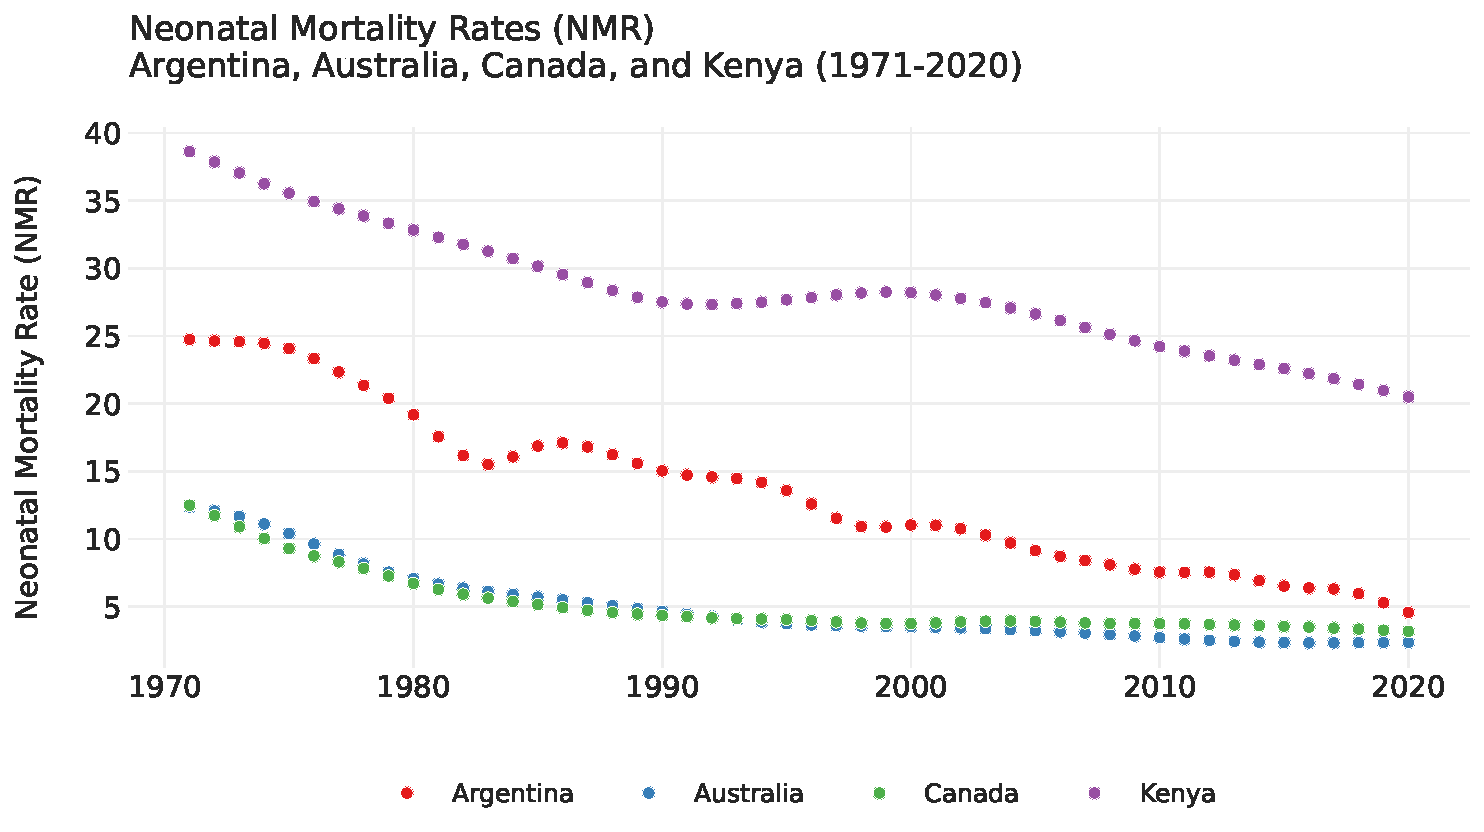
\includegraphics{firehose_files/figure-pdf/cell-33-output-2.pdf}

}

\end{figure}

\bookmarksetup{startatroot}

\hypertarget{references}{%
\chapter*{References}\label{references}}
\addcontentsline{toc}{chapter}{References}

\markboth{References}{References}

\hypertarget{refs}{}
\begin{CSLReferences}{0}{0}
\end{CSLReferences}



\end{document}
